%%
%% This is file `sample-sigconf.tex',
%% generated with the docstrip utility.
%%
%% The original source files were:
%%
%% samples.dtx  (with options: `sigconf')
%% 
%% IMPORTANT NOTICE:
%% 
%% For the copyright see the source file.
%% 
%% Any modified versions of this file must be renamed
%% with new filenames distinct from sample-sigconf.tex.
%% 
%% For distribution of the original source see the terms
%% for copying and modification in the file samples.dtx.
%% 
%% This generated file may be distributed as long as the
%% original source files, as listed above, are part of the
%% same distribution. (The sources need not necessarily be
%% in the same archive or directory.)
%%
%%%% Proceedings format for most of ACM conferences (with the exceptions listed below) and all ICPS volumes.
\documentclass[sigconf,nonacm,11pt]{acmart}
%%%% As of March 2017, [siggraph] is no longer used. Please use sigconf (above) for SIGGRAPH conferences.

%%%% Proceedings format for SIGPLAN conferences 
% \documentclass[sigplan, anonymous, review]{acmart}

%%%% Proceedings format for SIGCHI conferences
% \documentclass[sigchi, review]{acmart}

%%%% To use the SIGCHI extended abstract template, please visit
% https://www.overleaf.com/read/zzzfqvkmrfzn

% [ packages ] --------------------------------------------
% packages go here
% [ /packages ] -------------------------------------------

%%
%% \BibTeX command to typeset BibTeX logo in the docs
\AtBeginDocument{%
  \providecommand\BibTeX{{%
    \normalfont B\kern-0.5em{\scshape i\kern-0.25em b}\kern-0.8em\TeX}}}

\graphicspath{{fig/}{./}}

%%TC:ignore
%% Rights management information.  This information is sent to you
%% when you complete the rights form.  These commands have SAMPLE
%% values in them; it is your responsibility as an author to replace
%% the commands and values with those provided to you when you
%% complete the rights form.
\copyrightyear{2021}
\acmYear{2021}
\setcopyright{rightsretained}

%% These commands are for a PROCEEDINGS abstract or paper.
\acmConference{CSE6242}
\acmDOI{Data and Visual Analytics}
\acmISBN{}
\acmBooktitle{}
%%TC:endignore

%%
%% Submission ID.
%% Use this when submitting an article to a sponsored event. You'll
%% receive a unique submission ID from the organizers
%% of the event, and this ID should be used as the parameter to this command.
%%\acmSubmissionID{123-A56-BU3}

%%
%% The majority of ACM publications use numbered citations and
%% references.  The command \citestyle{authoryear} switches to the
%% "author year" style.
%%
%% If you are preparing content for an event
%% sponsored by ACM SIGGRAPH, you must use the "author year" style of
%% citations and references.
%% Uncommenting
%% the next command will enable that style.
%%\citestyle{acmauthoryear}

%%
%% end of the preamble, start of the body of the document source.
\begin{document}

%%
%% The "title" command has an optional parameter,
%% allowing the author to define a "short title" to be used in page headers.

\title{Real Estate Price: Economic and Ecologic Perspectives}
%%
%% The "author" command and its associated commands are used to define
%% the authors and their affiliations.
%% Of note is the shared affiliation of the first two authors, and the
%% "authornote" and "authornotemark" commands
%% used to denote shared contribution to the research.

%%TC:ignore

\author{Seth Caldwell}
\email{scaldwell36@gatech.edu}
\affiliation{%
  \institution{Georgia Institute of Technology}
}

\author{Muhammad Jarir Kanji}
\email{mkanji3@gatech.edu}
\affiliation{%
  \institution{Georgia Institute of Technology}
}

\author{James Mabry}
\email{jmabry9@gatech.edu}
\affiliation{%
  \institution{Georgia Institute of Technology}
}

\author{Jordan Nelson}
\email{jnelson300@gatech.edu}
\affiliation{%
  \institution{Georgia Institute of Technology}
}

\author{Guenter Roehrich}
\email{groehrich3@gatech.edu}
\affiliation{%
  \institution{Georgia Institute of Technology}
}

\author{Daemin Song}
\email{dsong74@gatech.edu}
\affiliation{%
  \institution{Georgia Institute of Technology}
}

% Short list on each page
\renewcommand{\shortauthors}{CS-6242 Team 054}

%%
%% The abstract is a short summary of the work to be presented in the
%% article.
%\begin{abstract}
%Based on county level data for all states of the United States of America, this article analyzed the relationship between the American real estate market and datasets covering economic as well as ecologic aspects.
%Other than existing analysis on this topic, this approach considers the prediction of prices not solely based on economic factors, but also takes environmental aspects into account.

% gist: homeownership is an important savings vehicle for building wealth and preparing for retirement in the US. it's becoming increasingly unobtainable for most households, and it's driven by factors such as internal features of the home as well as external municipal, socioeconomic, and ecological factors. households can currently get point-in-time home price estimates from services such as zillow, but much real estate industry historical data is walled off by trade groups. we're hoping to address the uncertainty involved in residential real estate purchasing by modeling home (listing?) prices using current residential listing data on Zillow and data capturing externalities (such as community socioeconomic and ecological factors) to provide transparent home price estimates for buyers and sellers. additionally, while we don't have historical home sales data, we will have historical socioeconomic and ecological data. so once we get a sense of the association between these factors and home prices (over time?), we can forecast short-term future trends for these factors to identify how home prices may change in the short-term.
%\end{abstract}

%\keywords{Real Estate, Regression, Time Series Analysis, Air Pollution}

%%TC:endignore

%% A "teaser" image appears between the author and affiliation
%% information and the body of the document, and typically spans the
%% page.
% \begin{teaserfigure}
%   \includegraphics[width=\textwidth]{sampleteaser}
%   \caption{Seattle Mariners at Spring Training, 2010.}
%   \Description{Enjoying the baseball game from the third-base
%   seats. Ichiro Suzuki preparing to bat.}
%   \label{fig:teaser}
% \end{teaserfigure}

\maketitle
%%TC:endignore

\section{Hi Team, start here}
[ Q's removed and inserted below ]
Hi Guys. This is just a copied version of the template we (should?) use - it is linked in the project requirement doc (Prof. Polo's).\newline
i'm also putting questions/things that i'm not sure about in three parentheses

\section{Problem Definition}
While the subprime mortgage crisis illuminated some risks, homeownership remains the preeminent savings vehicle for low- and moderate-income households to establish substantial savings, with an internal rate of return outpacing the stock market in a "typical" market \cite{Goodman2018}. Unfortunately, households face increasing difficulty in achieving homeownership due to incomes that have not kept pace with appreciating home prices, lack of housing inventory, and uncertainty in the homebuying process with commercial real estate price estimators operating as black boxes and the real estate industry controlling the data rather closely.

\section{Proposal}

\textbf{[1. What are you trying to do? Articulate your objectives using absolutely no jargon.]}
This project endeavors to address the difficulty of uncertainty by predicting current prices for the US residential real estate market (((and forecasting how those prices might change in the short term))). By blending real estate listings to capture internal features of a home with external features consisting of socioeconomic and ecological features of the community a home is situated in, the project will visualize the results to give users a transparent price model as well as how these factors vary by geographic region. For this purpose, we particularly focus on the overall air quality measure (AQ) or AQ index (AQI) and the amount of emitted particulate matter (PM). By understanding the influence of these factors and visualizing them geographically, the project will equip homebuyers with the ability to focus their search. Moreover, given historical data for these externalities, the project will provide homebuyers with historical context and possibly even short-term forecasts.
%Too far in the modelling topic, should not be in this paper (guenter - I wrote this paragraph earlier myself ;) )This will be accomplished through the application of multiple linear regression on the one hand, and time series analysis for factor prediction on the other hand. The underlying factors do cover a range of different data sets: Historic and current real estate prices obtained from Zillow.com (and/or related APIs), Salary data as well as education quality are another source of data that is added to build a more comprehensive regression model. In order to add another data dimension to the model, air quality measures are used to contribute the ecologic component of our prediction model. For this purpose we particularly focus on the overall air quality measure (AQ) or the AQ index (AQI) and the amount of emitted particular matter (PM).\newline

\textbf{[2. How is it done today; what are the limits of current practice?]}
%The US real estate market is a very competitive environment, hence attracting researchers to analyze its behavior both from academic, policy-driven perspectives as well as commercial perspectives.%
%While there is research on the impact of surrounding production activity on related real estate \cite{Nesticò2020}[nes], there are also more generic approaches looking at the impact of haze or the amount of ozone \cite{Anselin2006}[ans] on the real estate market. The pricing impact of particular matter (as a measure of air quality) was conducted earlier in the 2000s, investigating the described relationship for US metro areas [bay]. Recent approaches do investigate different angles of this complex topic of real estate evaluation, however do not particularly focus on providing insight and means to interactively identify areas that provide both, reasonable pricing and a sustainable environment to live in.
Households can use commercial tools like Zillow to obtain current home price estimates. These estimates operate as black-box algorithms that spit out a point-in-time price without context or consideration for short-term changes.
%Additionally, lack of access to historical real estate transaction data (which is held and controlled by individual MLIS trade groups around the country) presents a challenge to households (((right? -> but to us as well))).%

Existing academic approaches to residential real estate pricing primarily perform regression- and tree-based models with variables closely tied to the properties' attributes (e.g. number of rooms or age of the house) \cite{Kim2003} \cite{Ceh2018} \cite{Manjuna2017}. Alternative approaches explore communities' education qualities on the real estate market, which yields significant results; however, they only consider a relatively isolated viewpoint \cite{Fleishman2017} \cite{Seo2009}.

Other research focuses on ecological aspects. Existing literature notes that ecological degradation carries a quantifiable cost that is often overlooked (because it is not sold or traded) but nonetheless harms household and national wealth.

China's case is instructive, as it has experienced over the past few decades both a robust housing boom as well as increasing levels of particulate pollution (due to an economic boom propelled by heavy industry). These dual phenomena have garnered extensive interest in the effects of environmental factors on real estate prices \cite{Zheng2014} \cite{Mei2020}. While underlying studies often refer to and analyze a wider term of air pollution, an alternative focus on fine particulate matter ($PM_{2.5 }$) in other cases is also observed \cite{Chen2017} \cite{Chen2019} \cite{Wang2021} \cite{Sun2020} \cite{Dai2020}. These studies caution us to control for endogeneity issues (due to missing variables and reverse causality as home prices naturally increase in areas characterized by high economical productivity associated with ecologically harmful heavy industry) that cause ordinary least squares (OLS) estimation to bias the ecological covariate to zero \cite{Zheng2014} \cite{Chen2017} \cite{Chen2019}.\newline However, the Chinese experience does not translate perfectly to the US experience. In particular, these studies ignore individual home features because newly built commodity housing accounts for the majority (more than 70\%) of real estate market activity in China \cite{Chen2017}. Additionally, no reliable second-hand transaction data exists for the Chinese real estate market \cite{Zheng2014}.

Around the world, other studies have used multiple regression to explain the relationship between purchase price and "ecosystem disservice" in Italy. The authors further attempt to forecast home depreciation due to air pollution \cite{Nestico2020}. However, the sample size is comparatively small (consisting of just 60 residential sales over three years), and the authors neglect to use the log-linear functional form, which much literature recommends for hedonic price modeling to mitigate heteroscedasticity \cite{Morano2019} \cite{Fletcher2000} \cite{Cassel1985}. In Colombia, research leverages both stages of Rosen's hedonic pricing framework %(first-stage Hedonic Price Function estimation and Second Stage estimation of demand for a specific feature obtained by combining first-stage hedonic price estimations with socioeconomic data reflective of household preferences) %
\cite{Rosen1974} in a log-linear regression model showing the positive effect of good AQ on home prices \cite{Carriazo2018}.

Literature is sparse on the effects of AQ on the US real estate market and primarily uses AQ as a vehicle for illustrating methodological challenges in the hedonic pricing model. For instance, interpolating data collected at geographically fixed sampling stations to geographically distributed phenomena \cite{Anselin2006} and illustrating the effect of mobility constraint on marginal willingness to pay for community factors such as clean air \cite{Bayer2009}.

\textbf{[3. What's new in your approach? Why will it be successful?]}
Providing a transparent residential real estate pricing model \textendash as well as insight into potential short-term changes \textendash makes this project novel. 

This project will overcome the challenge presented by a lack of access to historical real estate transaction data by creating an enriched composite dataset of several data sources. Specifically, socioeconomic and ecological data will be obtained from official sources (e.g. US government agencies and open data portals), and prices and internal features of homes currently listed will be scraped from Zillow.

We anticipate that the project will apply the flexible multiple regression framework to model home prices \cite{James2014} \cite{James2014:LinearRegression}. It may be beneficial to explore Bayesian regression to more clearly quantify the uncertainty of our estimates and/or if we come across reliable historical data \cite{Gelman2014:BayesianLinReg}. Because the real estate data can come from different regional groups (e.g., different metro areas, different states, etc.), it also may be beneficial to explore multilevel/hierarchical approaches \cite{Gelman2007:MultilevelLinReg} \cite{Gelman2014:HierarchicalModels} \cite{Gelman2014:HierarchicalLinearModels} and/or evolutionary approaches \cite{Morano2019} to fit a model that services multiple regional groups.

And it certainly will be critical to heed the lessons from existing literature to adapt multiple regression to some of the idiosyncracies of real estate valuation \cite{Rosen1974} \cite{Ceh2018} \cite{Bin2004}. Specifically, literature on hedonic regression for real estate prescribes the log-linear functional form to mitigate heteroscedasticity that can be present in modeling real estate transactions \cite{Morano2019} \cite{Fletcher2000} \cite{Cassel1985}. Some literature modeling home prices and ecological factors finds that treating ecological variables as categorical rather than quantitative yields superior results \cite{Anselin2006}. If the data spans geographic regions, existing literature provides some guidance for exploring multilevel models \cite{Chen2017} or evolutionary algorithms \cite{Morano2019}. Much research modeling home values and environmental factors shares the shortcoming that internal features of homes are treated as fixed, more or less identical commodities \cite{Chen2017} \cite{Chen2019} \cite{Nestico2020} \cite{Bayer2009} \cite{Wang2021} \cite{Mei2020} \cite{Sun2020} \cite{Dai2020} \cite{Kim2003} \cite{Zheng2014}. Additionally, some literature finds that the normal error term assumed in most hedonic regression modeling of real estate prices may be inaccurate \cite{Francke2017}; in these cases, it may be worth exploring heavier-tailed variants (such as the t-distribution) for robustness against outliers \cite{Francke2017} \cite{Gelman2007:GLM}.

This approach does not only combines a variety of datasets, but uses different algorithms to make predictions and further identify relatively undervalued real estate. Underlying data is not only obtained from official sources (e.g. governmental, census), but obtained by scraping web resources. This allows more detailed, even county-level, analysis. To enhance the success of this idea, the dataset which is based on real estate, education and demographic data will further be extended through an environmental aspect, air quality measures. In order to obtain most recent and future values for AQ, time series models are used to predict the average air quality factor.
AQ will be measured through the AQI as well as the amount of particulate matter, expressed similar to the figure in the appendix.

\textbf{[4. Who cares?]}
Households seeking to purchase a house will benefit from transparent price modeling along with the visualization of external factors.
%This idea may be a key centerpiece in the decision making process, whether to buy real estate in a specific area (to a given price), or not. This approach not only provides the monetary view onto the real estate value, but also introduces the dimension of the environmental impact on its residents.

\textbf{[5. If you're successful, what difference and impact will it make, and how do you measure them (e.g., via user studies, experiments, ground truth data, etc.)?]}
This projects aims at providing users with both an accurate, transparent view with regard to the value of real estate. This value is defined through the quantitative measures closely tied to the property; however it also takes into account external features. Eventually, an undervalued real estate will benefit its potential buyers.

\textbf{[6. What are the risks and payoffs?]}
A potential risk is that environmental aspects do not explain significant variability in home prices; however, the project aims at providing this additional view point to support a potential buying decision.

\textbf{[7. How much will it cost?]}
No monetary costs are anticipated; team time investment is the primary cost.
%This is a class project, therefore the time invested in the project can be seen as the project cost.

\textbf{[8. How long will it take? (Need to include milestones/plan of action)]}
The project is anticipated to take no more than two months. There are three major milestones: \textbf{(1)} As real estate listing data is unavailable as simple downloads or API portals, these data must be scraped, cleaned, and integrated with the external socioeconomic and AQ data (which can be downloaded); \textbf{(2)} analyzing the data to model home prices on home features and external factors; \textbf{(3)} deploying the model, consisting of a geographic visualization of the results and a web interface.

\textbf{[9. What are the midterm and final "exams" to check for success? How will progress be measured?]}
The three milestones above will serve as progress guideposts. The team meets weekly to review progress against these milestones, aided by a GitHub Project board.

\section{Plan of Activities}
All team members have contributed comparably. We anticipate that this will continue to be the case.
\begin{enumerate}
  \item{\textbf{2021-02-28}: Brainstorm topics, divide into two groups to collect sample data and rough prototypes for two top topics (\textit{all})}
  \item{\textbf{2021-03-12}: Proposal and presentation}
  \begin{itemize}
    \item{Research (\textit{all})}
    \item{Proposal document (\textit{Guenter, Jordy, Muhammad})}
    \item{Proposal video (\textit{Daemin})}
  \end{itemize}
  \item{\textbf{2021-03-19}: Data collection, cleaning, storage}
  \begin{itemize}
    \item{Real estate, salary, \& education data (\textit{James, Seth, Daemin})}
    \item{Air quality data (\textit{Guenter, Jordy, Muhammad})}
    \item{Data storage (\textit{James})}
  \end{itemize}
  \item{\textbf{2021-04-01}: Modeling (\textit{all})}
  \begin{itemize}
    \item{Exploratory analysis (\textit{all})}
    \item{Model building and selection (\textit{all})}
  \end{itemize}
  \item{\textbf{2021-04-02}: Progress report (\textit{all})}
  \item{\textbf{2021-04-15}: Deployment}
  \begin{itemize}
    \item{Visualization (\textit{all})}
    \item{Web interface (\textit{all})}
  \end{itemize}
  \item{\textbf{2021-04-23}: Final poster and presentation (\textit{all})}
\end{enumerate}

\pagebreak

\appendix
\section{Appendix}

\begin{figure}[!h]
    \centering
    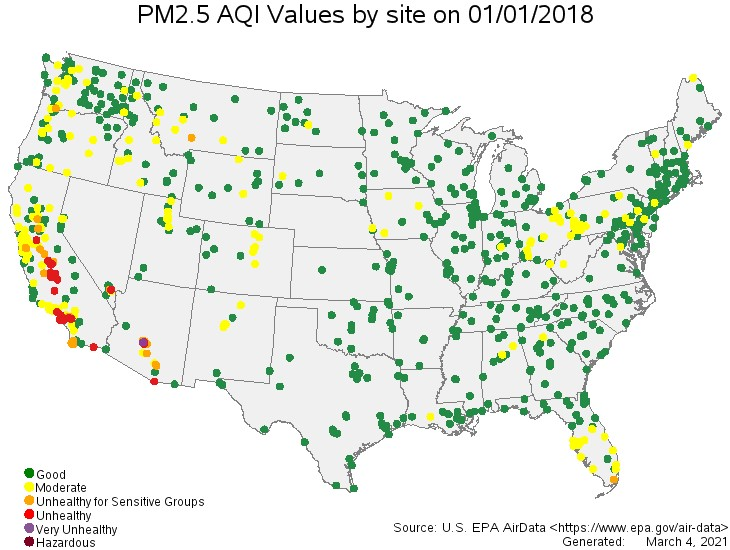
\includegraphics[scale=0.4]{AQ_US_2018.jpg}
    \caption{PM2.5 AQI Values}
\end{figure}

\pagebreak

% %%
% %% The acknowledgments section is defined using the "acks" environment
% %% (and NOT an unnumbered section). This ensures the proper
% %% identification of the section in the article metadata, and the
% %% consistent spelling of the heading.
% \begin{acks}
% To Robert, for the bagels and explaining CMYK and color spaces.
% \end{acks}

%%
%% The next two lines define the bibliography style to be used, and
%% the bibliography file.
\bibliographystyle{ACM-Reference-Format}
\bibliography{references}


%%
%% If your work has an appendix, this is the place to put it.
\appendix

% \section{Research Methods}

% \subsection{Part One}

% Lorem ipsum dolor sit amet, consectetur adipiscing elit. Morbi
% malesuada, quam in pulvinar varius, metus nunc fermentum urna, id
% sollicitudin purus odio sit amet enim. Aliquam ullamcorper eu ipsum
% vel mollis. Curabitur quis dictum nisl. Phasellus vel semper risus, et
% lacinia dolor. Integer ultricies commodo sem nec semper.

% \subsection{Part Two}

% Etiam commodo feugiat nisl pulvinar pellentesque. Etiam auctor sodales
% ligula, non varius nibh pulvinar semper. Suspendisse nec lectus non
% ipsum convallis congue hendrerit vitae sapien. Donec at laoreet
% eros. Vivamus non purus placerat, scelerisque diam eu, cursus
% ante. Etiam aliquam tortor auctor efficitur mattis.

% \section{Online Resources}

% Nam id fermentum dui. Suspendisse sagittis tortor a nulla mollis, in
% pulvinar ex pretium. Sed interdum orci quis metus euismod, et sagittis
% enim maximus. Vestibulum gravida massa ut felis suscipit
% congue. Quisque mattis elit a risus ultrices commodo venenatis eget
% dui. Etiam sagittis eleifend elementum.

% Nam interdum magna at lectus dignissim, ac dignissim lorem
% rhoncus. Maecenas eu arcu ac neque placerat aliquam. Nunc pulvinar
% massa et mattis lacinia.

\end{document}
\endinput
%%
%% End of file `sample-sigconf.tex'.
